\documentclass{article}
\usepackage{mathtools, amssymb, amsthm, tikz}

\title{Homwork 4 \\ CMPSC 465}
\author{Nimai Patel}

\begin{document}

\section {Depth-First Search}

Perform depth-first search on each of the following graphs; whenever there’s a
choice of vertices, pick the one that is alphabetically first. Classify each
edge as a tree edge, forward edge, back edge, or cross edge, and give the pre
and post number of each vertex.

\begin{enumerate}
        \item First Graph: \\
              \begin{center}
                      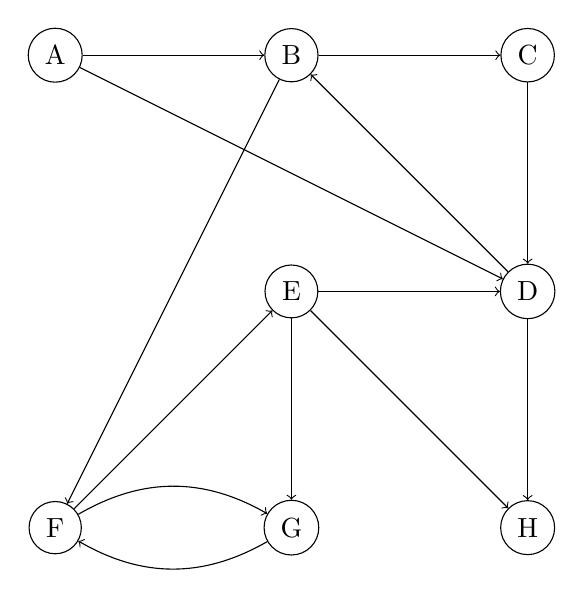
\begin{tikzpicture}
                              \node[draw,circle] (A) at (0,0) {A};
                              \node[draw,circle] (B) at (3,0) {B};
                              \node[draw,circle] (C) at (6,0) {C};
                              \node[draw,circle] (D) at (6,-3) {D};
                              \node[draw,circle] (E) at (3,-3) {E};
                              \node[draw,circle] (F) at (0,-6) {F};
                              \node[draw,circle] (G) at (3,-6) {G};
                              \node[draw,circle] (H) at (6,-6) {H};

                              \draw[->] (A) -- (B);
                              \draw[->] (A) -- (D);
                              \draw[->] (B) -- (C);
                              \draw[->] (B) -- (F);
                              \draw[->] (C) -- (D);
                              \draw[->] (D) -- (B);
                              \draw[->] (D) -- (H);
                              \draw[->] (E) -- (D);
                              \draw[->] (E) -- (H);
                              \draw[->] (E) -- (G);
                              \draw[->] (F) -- (E);
                              \draw[->] (F) to [bend left] (G);
                              \draw[->] (G) to [bend left] (F);
                      \end{tikzpicture}
              \end{center}
        \item nice
\end{enumerate}

\end{document}